\section{Introduction}

    %* show the problem
    %* introduce the idea
    %* contributions?

	% motivation
	A service robot operating in human environments should be able to perform complex tasks in a variety of conditions. This requires good perception capabilities, one of which is to reliably detect and recognize objects in the scene.

    % introduce the problem
    Many state-of-the-art object recognition systems have been developed using a variety of feature extraction techniques. Despite the fact that some of them have been very successful, we still cannot say that the problem of object recognition has been solved. We claim that the reason for that is already included in the problem formulation. Given static images there are cases where it is impossible to recognize the object as it may appear ambiguous with respect to another object(see~\figref{fig:pr2}). One of the reasons for that is that distinctive features may be hidden due to the pose of the object. 
    
	% general approach    
There has been different approaches to tackle this problem. One of them is active perception, where the robot is intelligently moving around the scene to reveal more information of the object it is looking for. In this paper we present another approach where the robot interacts with the scene in order to reduce the uncertainty of the object it sees.
    
    % introduce the idea
    We take advantage of robot's manipulation capabilities and apply them in the domain of object recognition. In our approach we tackle interactive object recognition problem where we look for the action that will minimize the expected entropy over objects distribution. Therefore we want to be optimal in the number of actions that will lead us to successful object recognition.

    % contributions
    The key contributions of our approach are that (a) to the best of our knowledge, we are first to introduce the idea of a robot interacting with the scene in order to improve object recognition, (b) our approach takes into account a probabilistic object recognition model that is agnostic to the feature type, (c) we present a probabilistic action selection model that reasons about the most informative action which leads to optimality in the number of actions to recognize the object.

    \setlength{\tabcolsep}{0.1em}
    \begin{figure}[ht]
    \begin{tabular}{cccc}
    \multicolumn{2}{c}{\multirow{-5}{*}{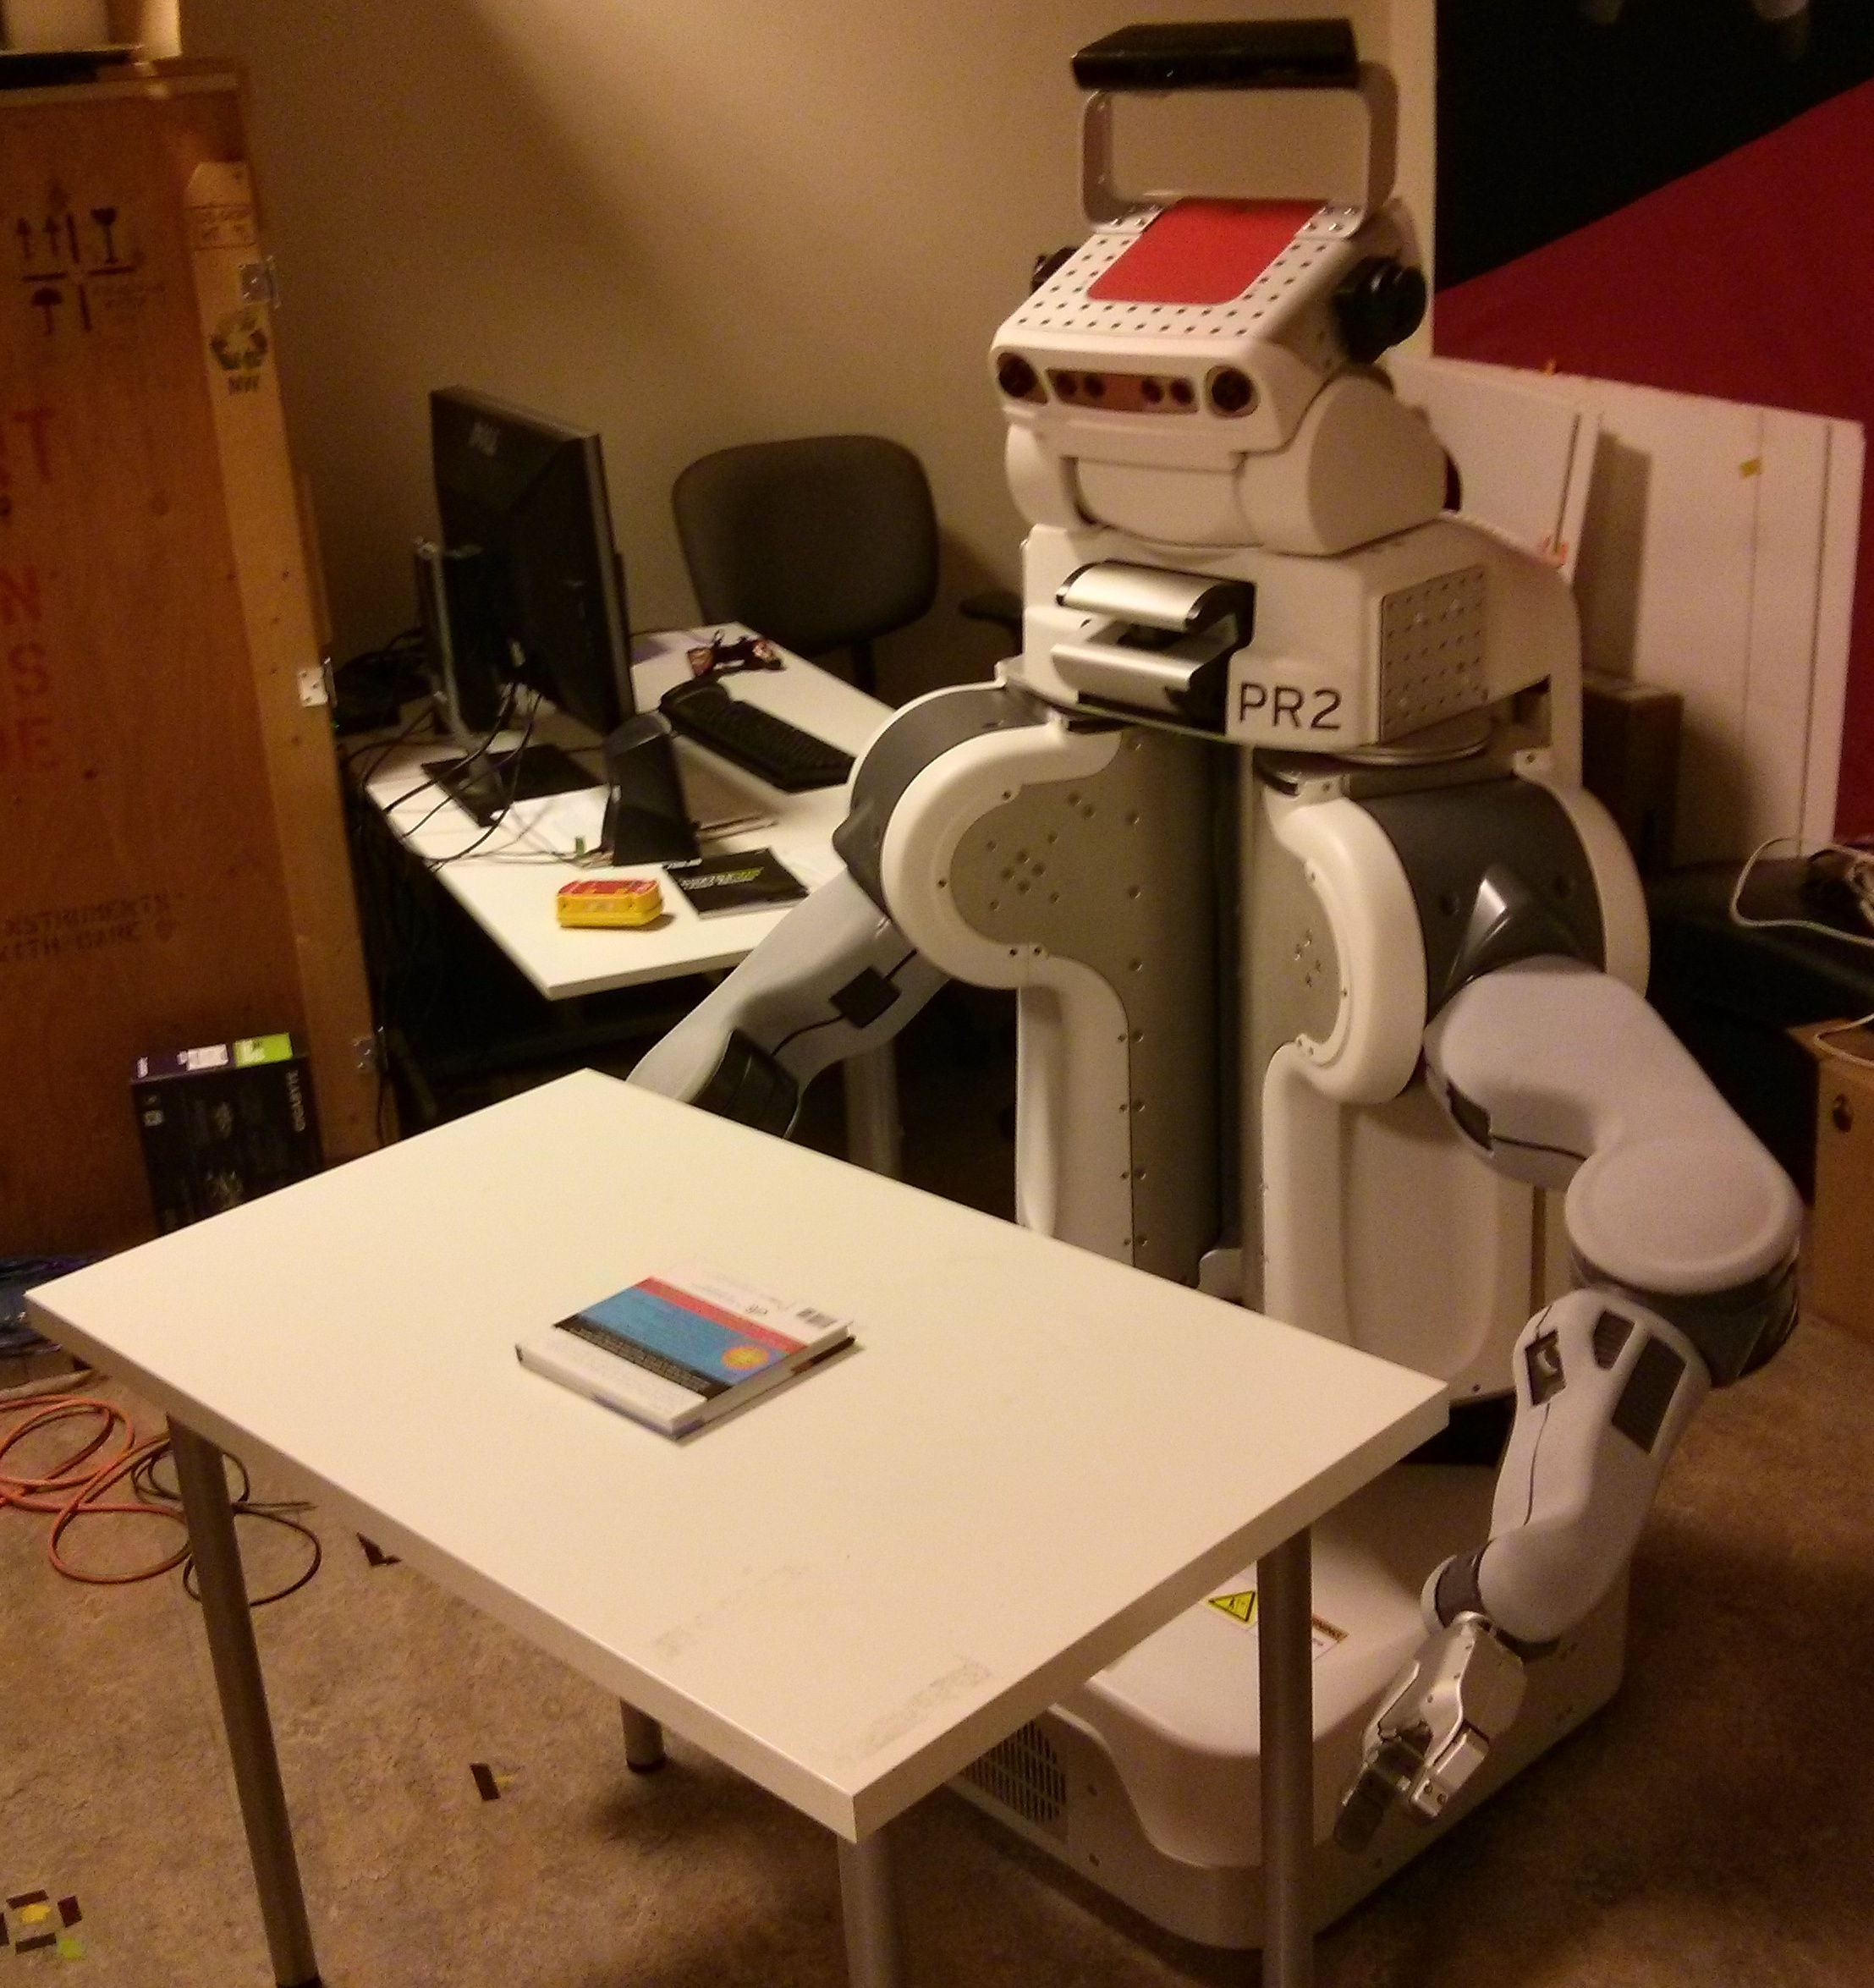
\includegraphics[width=0.46\columnwidth]{pics/pr2_init.jpg}}} & 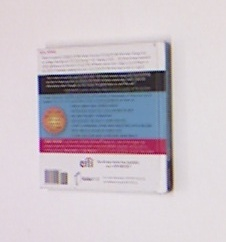
\includegraphics[width=0.23\columnwidth]{pics/first_back.jpg} 
    &
\includegraphics[width=0.23\columnwidth]{pics/first_cover1.jpg} \\
    \multicolumn{2}{c}{} & 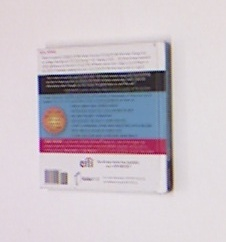
\includegraphics[width=0.23\columnwidth]{pics/first_back.jpg} 
    &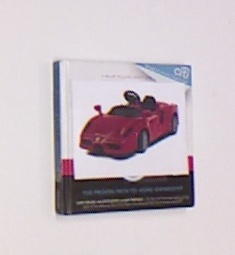
\includegraphics[width=0.23\columnwidth]{pics/first_cover2.jpg} \\
    \multicolumn{2}{c}{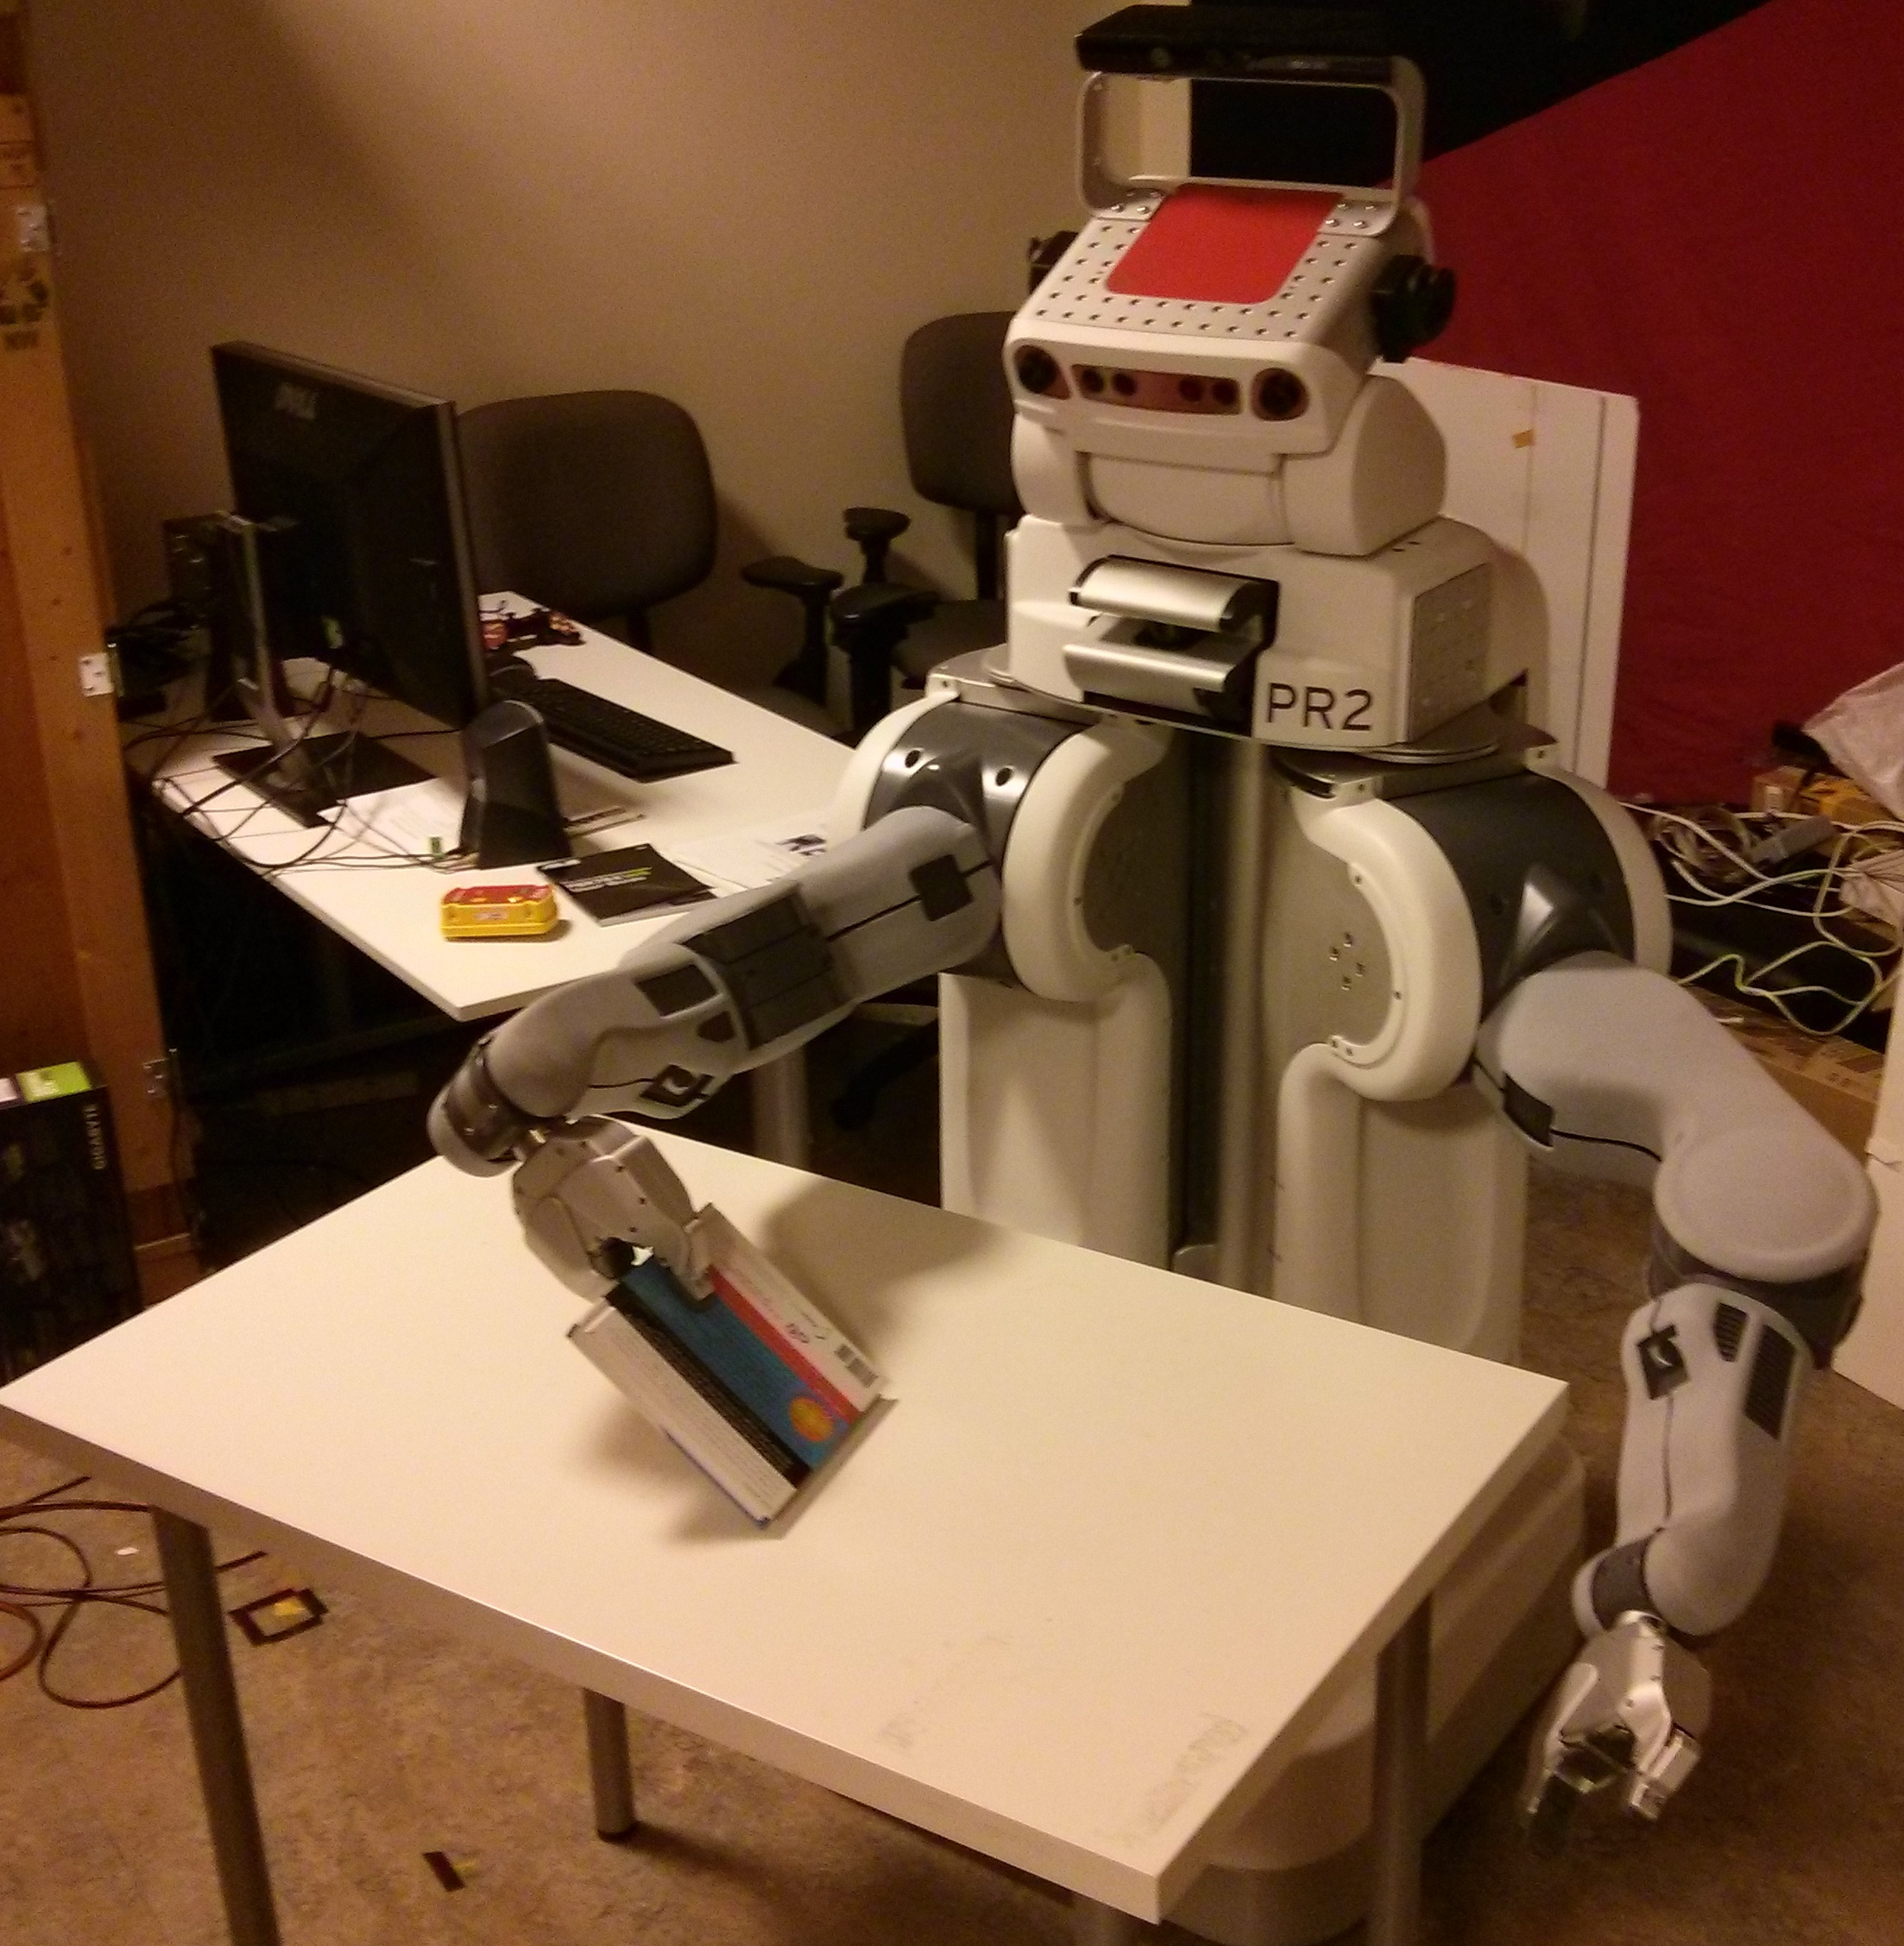
\includegraphics[width=0.45\columnwidth]{pics/pr2_grasp.jpg}}
    & \multicolumn{2}{c}{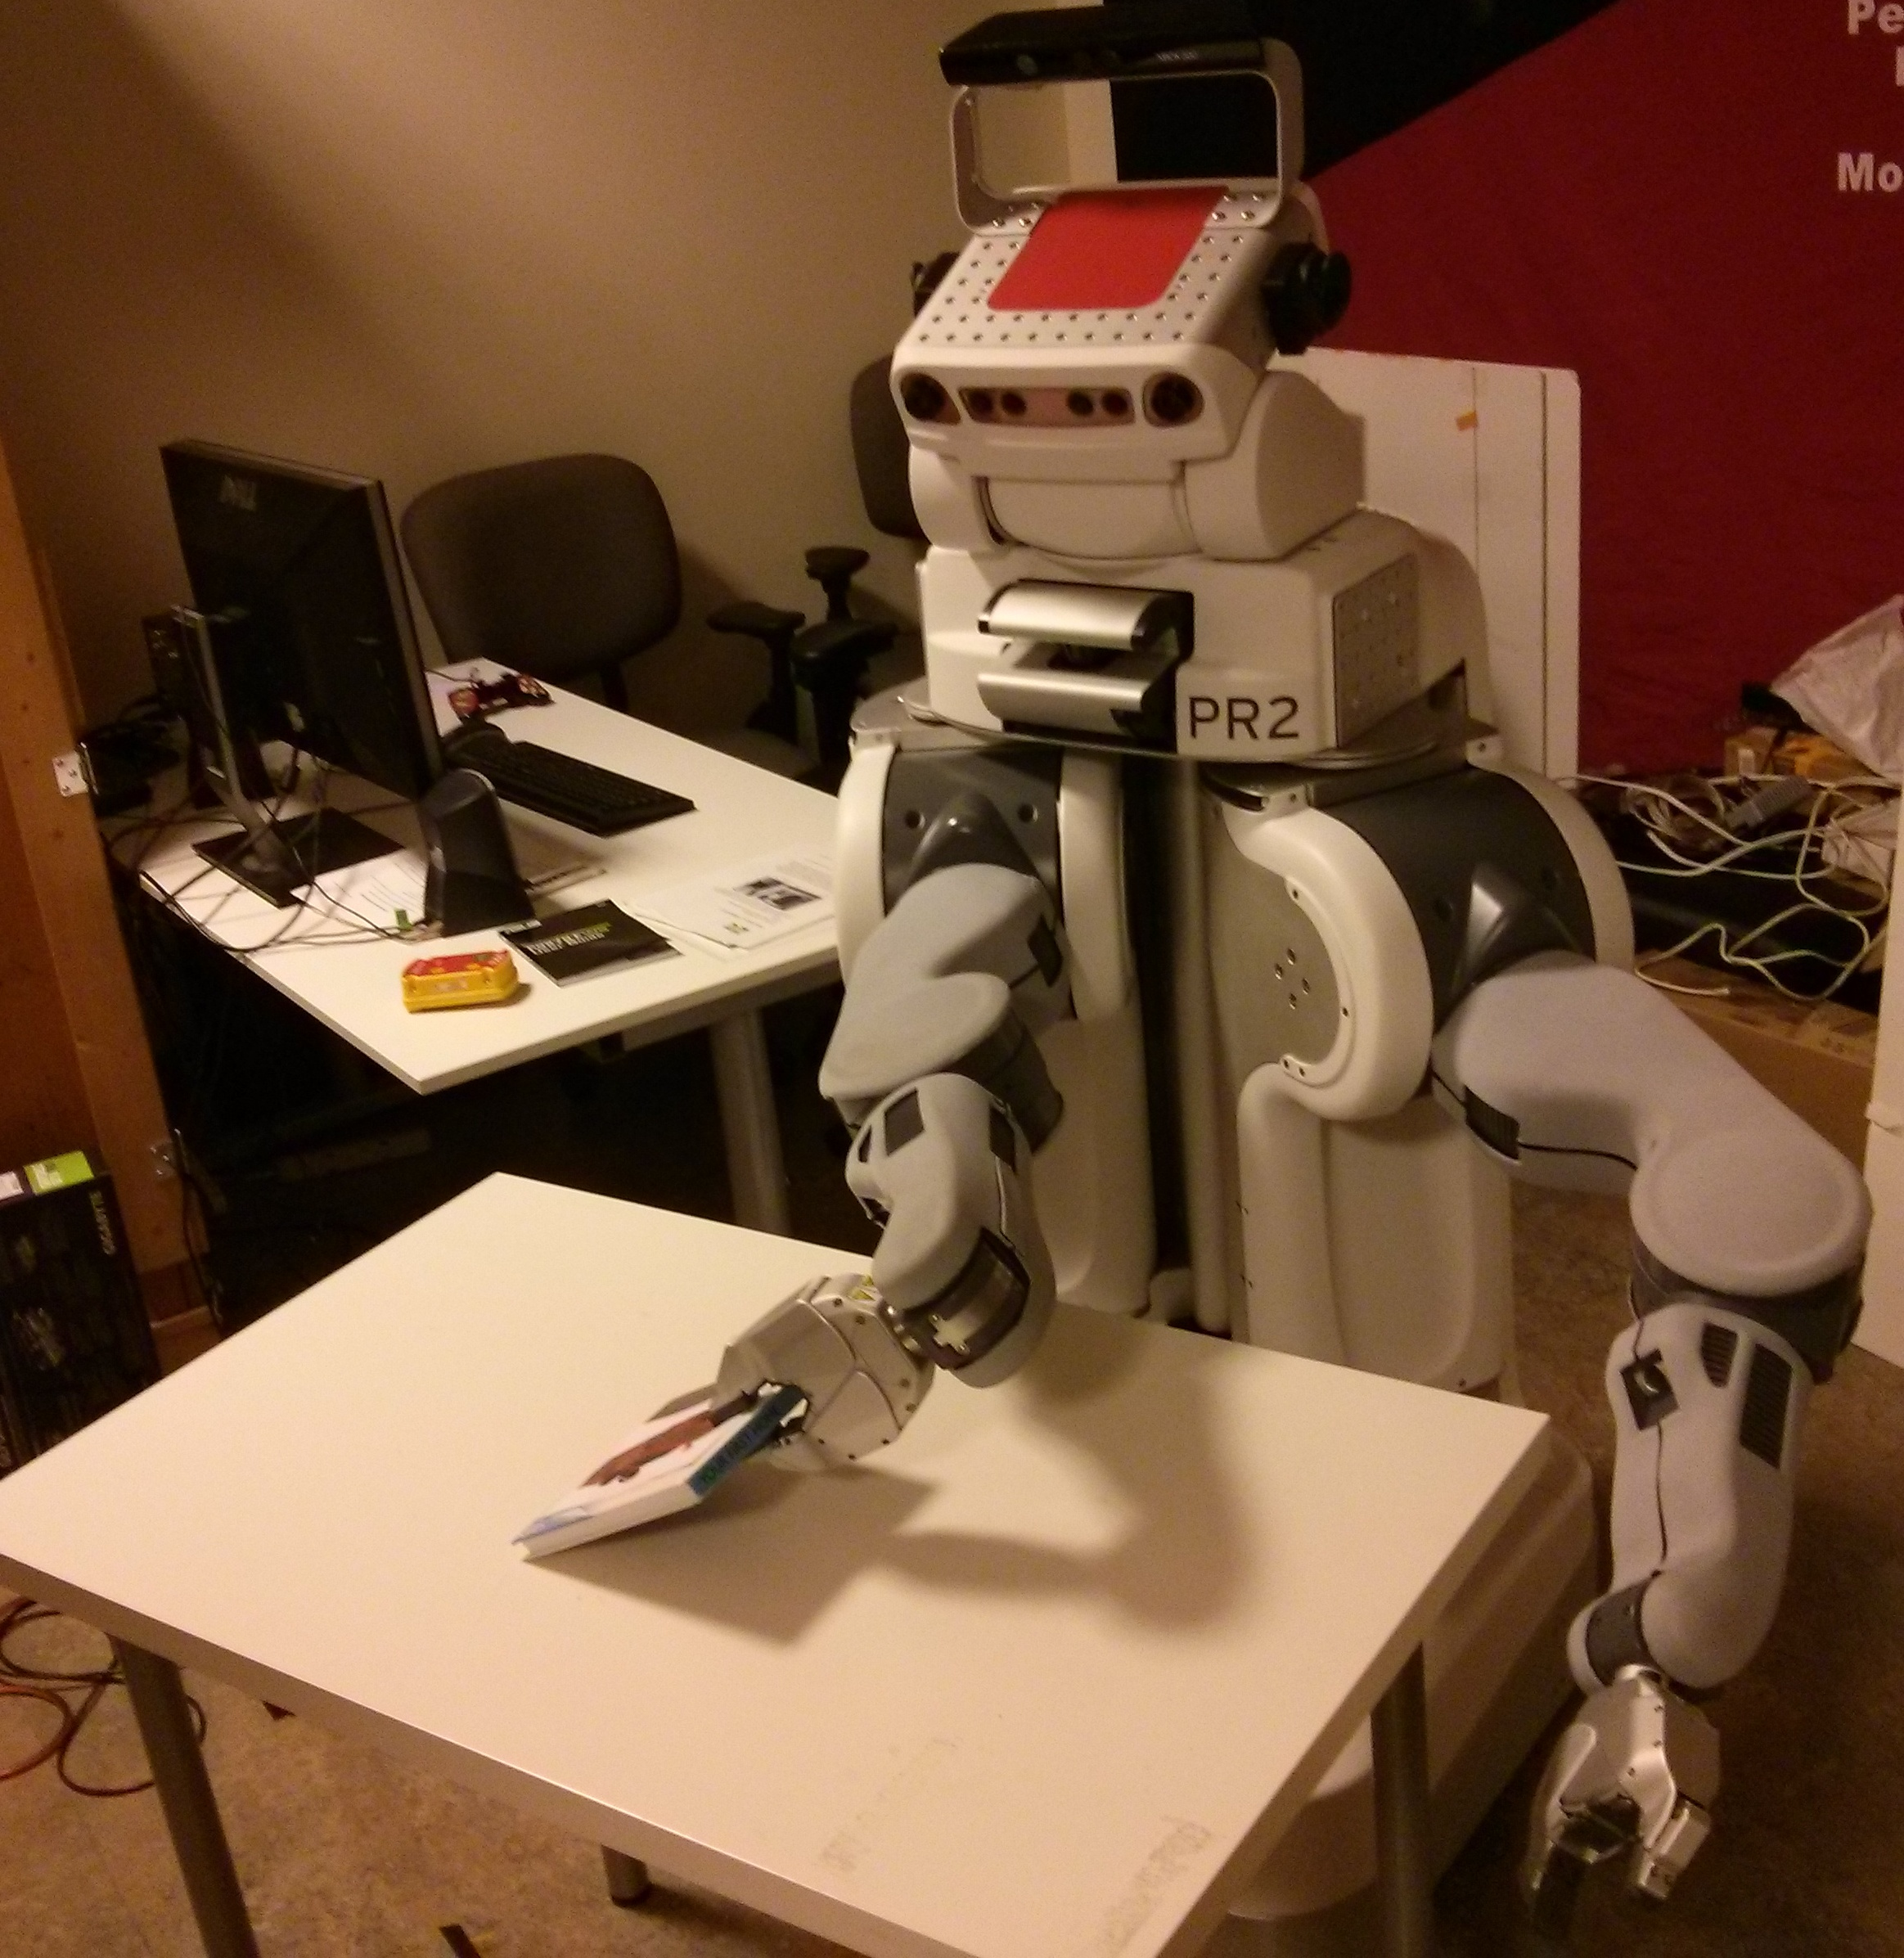
\includegraphics[width=0.45\columnwidth]{pics/pr2_rotate.jpg}}
    \end{tabular}
    \caption{Top-left: The service robot PR2 trying to recognize a book based on the back. Database of objects consists of book 1 (top-right, NE and NW) and book 2, (top-right, SE and SW) that look the same from the back. PR2 has to take the optimal action in order to recognize which book it is. In this case it means it flips it over(bottom-left, bottom-right).}
    \label{fig:pr2}
    \end{figure}

    %contributions
    %* novel probabilistic model for object recognition
    %* action selection probabilistic algorithm to pick the optimal action in order to recognize the object
